\documentclass[hidelinks,12pt,a4paper]{book}
%\usepackage{booksprint}
\usepackage[T1]{fontenc}
\usepackage[utf8]{inputenc}
\usepackage{graphicx}
\usepackage{authblk}
\usepackage{hyperref}
\usepackage{subcaption}
\usepackage{enumitem}
\usepackage{xcolor}
\usepackage{outlines}
\usepackage[tikz]{bclogo}
\usepackage{tikz}
\usetikzlibrary{calc}
\usepackage{float}
\usepackage{lipsum}
\usepackage{subcaption}
\usepackage{environ}
\renewcommand{\labelitemii}{\textbullet}

%\usepackage[printonlyused,withpage]{acronym}
\usepackage[nolist,withpage]{acronym}
\usepackage{glossaries}
\usepackage{gincltex}
\usepackage{tabularx}
\usepackage[all]{nowidow}

\usepackage[style=numeric,natbib=true,backend=bibtex]{biblatex}
\makeatletter
\def\blx@maxline{77}
\makeatother

\usepackage{color}

\definecolor{pblue}{rgb}{0.13,0.13,1}
\definecolor{pgreen}{rgb}{0,0.5,0}
\definecolor{pred}{rgb}{0.9,0,0}
\definecolor{pgrey}{rgb}{0.46,0.45,0.48}

\usepackage{listings}
\lstset{language=Java,
  showspaces=false,
  showtabs=false,
  breaklines=true,
  showstringspaces=false,
  breakatwhitespace=true,
  commentstyle=\color{pgreen},
  keywordstyle=\color{pblue},
  stringstyle=\color{pred},
  basicstyle=\ttfamily,
  moredelim=[il][\textcolor{pgrey}]{\$\$},
  moredelim=[is][\textcolor{pgrey}]{\%\%}{\%\%}
}

\def\postbreak{%
  \raisebox{0ex}[0ex][0ex]{\ensuremath{\hookrightarrow\space}}}
  
\addbibresource{main.bib}
   
%\renewcommand{\familydefault}{\sfdefault}

\sloppy

\makeglossaries
\begin{document}
	

%-----------------------------------------
% Title, Table of Contents
%-----------------------------------------

\begin{titlepage}
	\centering
	
\includegraphics[width=0.25\textwidth]{figures/tu_logo}\par\vspace{1cm}
	{\scshape\LARGE Technische Universität Berlin \par}
	\vspace{0.75cm}
	
\includegraphics[width=0.3\textwidth]{figures/ise_logo}\par
    \vspace{0.25cm}
	{\normalsize Wirtschaftsinformatik - Information Systems Engineering \par}
    \vspace{0.5cm}
	{\scshape\Large Cloud Prototyping Project\par}
	\vspace{0.75cm}
	{\Large\itshape Darshan Mukund Hingu\par}
	{\Large\itshape Kevin Hudemann\par}
	{\Large\itshape Gerrit Janßen\par}
	{\Large\itshape Mukrram Ur Rahman\par}
	{\Large\itshape Muhammad Talal Saleem\par}
	{\Large\itshape Vinothkumar Nagasayanan\par}
	{\Large\itshape Ron Wierzchowski\par}
	\vfill
	Supervised By:\par
	Dominik \textsc{Ernst}\par
	Prof. Dr.-Ing. Stefan\textsc{ Tai}\par
	\vfill
	{\large \today\par}
\end{titlepage}

%\logos
\newpage
\thispagestyle{empty}
\mbox{}


\setcounter{secnumdepth}{4}
\setcounter{tocdepth}{3} 




%-----------------------------------------
% Content
%-----------------------------------------

\chapter*{Abstract}


\tableofcontents

% add here your parts of the documentation


\chapter{Introduction}




\section{Basics of Provenance Systems}
Provenance is simply data quality. Provenance is the relationship among all elements that contributed to the existence of a piece of data.The provenance of data focuses on the history of changes and movement of data. The history of data changes can include subsetting, formatting, transformation, semantic transformation, syntactic transformation and ingesting new data to the existing data. To maintain or proved the quality of data the lineage of the data needs to collected throughout the data transformational process. The metadata to ensure the quality of the data is to be generated in systematic function. All the information about the elements and the relationship among all the elements (sources, processing steps contextual information and dependencies) should include in the definition of provenance capturing. 


There are clear differences between process provenance (focusing on workflow execution and the execution environment) and data provenance (focusing on creation and transformation of data). Understanding the type of provenance information of interest and how it will be used can help inform the decision for how to capture the provenance information. The provenance of data can often be collected automatically by saving system logs for events, system inputs, and system outputs but this kind of the provenance does not capture the insight and the rational decision made by the system. 

In practical situations, it is not easy to completely capture all types of provenance information. Provenance information can be captured with varying levels of detail.  Provenance granularity describes the level of detail of the captured information. The level of provenance granularity is motivated by the use of the particular system.In this project, we are focused towards the data provenance mechanism and technique used to capture in a distributed setup.

\subsection{Purpose}
Capturing the process of formation of data in the IoT ecosystem is like three-folding the already data being generated by the sensor. So, there must a concrete reason for doing this. One simple answer to this is that the data in possession will support the ongoing analysis or some-what enhances the result once the results are completed.

Recall of the analytic process is one of the common purposes to capture provenance. Recall enables awareness and understanding of what processing went through and what task are pending. Recalling is important for analytic clarity and efficiency especially when the processing step is complex and interconnected to another component in the architecture. 

Another common purpose of provenance information is to reproduce previously obtain the result. This help to verify that the result is correct and can be trusted. Difference between the results after toggling environment and context parameter can be clearly seen resulting in choosing the best suitable parameter for the upcoming deployment.

Another purpose for provenance involves reviewing the processing step itself and the environment it was run on. This Meta-analysis of processes makes it possible to review and evaluate the step and decision made by the component for the creation of the data. Meta-analysis help to extract patterns and help to optimize performance and suggestion on the changes in real time if need be.

\subsection{Provenance in IoT}
Data in IoT ecosystem is produced in large velocity, volume, and variety. In order to examine and maintain the correctness of the data, provenance data systems are introduced to increase the authenticity. Due to the complicated structure of IoT pipeline in which data comes from distributed nodes across the architecture extremely hard to track manually provenance system is necessary for any sort of insurance on the existing data properties.

Numerous jobs applying complex operation on them are performed which is then propagated to produce some sort of insight from the data or maybe feed into a machine learning algorithm. Finding the reason for an anomaly or outlier from the huge chunk for the data scientist resulting in unexpected results can be a daunting task without capturing of provenance information. 

Debugging unexpected results can be narrow done to the components through which the data has gone through saving a lot of time.This help makes analytic decision which was unable to make without the help of the lineage of the data captured. In case of a distributed system where the data is digitally transformed and derived from numerous sources by applying complex function in various context can produce different results. The advantage of using provenance system with the existing system gives the ability to use the data produced by giving the user transparent view of the whole process and the underlying mechanism used to collect it across a different component of a data-processing workflow so the user knows how the data is molded before it reached to the endpoint.

Capturing provenance information in a distributed system gives insight not only to the data-dependencies but also for fault tolerance and usage statistics. Collection of provenance information is useful in many contexts, such as verifying result and explaining the existing of the item. Capturing provenance information for any specific workflow or process make the user of the data to easily follow the origin of the data. 


\subsection{Challenges}
Collecting provenance for any given system is a difficult task at hand and requires a deep understanding of the underlying architecture of the system to implement an efficient and useful provenance system. This includes taking into account that every architectural design in every situation is motivated by some core values behind that system which need to be taken into account when building a provenance system which tracks each and every movement of the system overall. There is a lot unanswered question provenance architect has to decide on before building a model which suit the system and fulfill the sole purpose it is built for. Typically, when talking about provenance in IoT domain where the addition of one component can scale the data generated exponential can cause disastrous effect if the decision is not made after suitable consideration and trade-off in mind. 

Provenance collecting for this kind of system must be able to scale to both large volumes of data and numerous operation to avoid being a bottleneck. Distributed pipeline are difficult to manage and control especially when there is a great chance of failure of the system and avoid running the provenance system when some component is not working correctly. This might corrupt the data and will produce gibberish data not useful for anyone.

Provenance system should consider the finer granularity in which it captures the transformation of data. Some component of the system is transparent in term of how the data is manipulated.  On the other hand, the black-box operator is not transparent enough and does not know how the transformation is taking place. Producing highly accurate provenance for this kind of operation requires specific techniques which incur time overhead to capture and there is a direct trade-off between the performance of the system.



\section{Related Work}




\section{Project Organization}

When starting this project as a team of equal students, the distribution of tasks was not trivial as we first had to come up with a problem, use-case and a general vision of what we wanted to achieve. 
Therefore initially everybody had to figure that out for themselves, before discussing it in the group and coming to an agreement.

After making these high-level decisions, tasked were started to be distributed based on personal preferences. 
The granularity of tasks was evolving over time, though quite differently for different tasks.
For example, it became clear at the beginning that we needed a simulation of a smart grid on which we could test our prototype, which resulted in rather precise implementation tasks early on. 
However, the design of the data model took more research and was also revised repeatedly, so that the first fine grained implementation tasks were started some weeks later.

After the first five weeks a scrumboard was introduced \cite{zenhub}. 
Before that, regular github issues were used to define task distribution. 
However, with ever more fine grained and interconnected implementation tasks, it became harder to keep the overview. 
The scrumboard therefore helped to keep a better overview and also subjectively increased the teams performance, especially once we started to set deadlines on a weekly basis.

The Following table was set before the midterm presentation to define responsibilities, especially when it comes to questions regarding the components from within the team as well as from outsiders.


\renewcommand{\arraystretch}{1.4}
\begin{center}
 \begin{tabular}{| m{18em} m{10em} |} 
 \hline
 Responsibility & Name  \\
 \hline\hline
 IoT Pipeline & Kevin \\ 
 \hline
Data Model + Provenance Collector & Mukrram \\
 \hline
 Backend & Vinoth, Mukrram \\
 \hline
 Databases & Talal \\
 \hline
 Frontend & Darshan \\ 
 \hline
 Deployment \& Testing & Gerrit \\
 \hline
Project Management & Ron \\
 \hline
\end{tabular}
\end{center}


\section{Use Case}

A smart grid is an electrical grid which includes a variety of operational and energy measures including smart meters, smart appliances, renewable energy resources, and energy efficient resources.
Electronic power conditioning and control of the production and distribution of electricity are important aspects of the smart grid. 
Providing reliability in smart grids are done using electronic control, metering, and monitoring. 
To motivate our design decisions we are looking at how a potential user would interact with our system. 
In this chapter we are looking at the Administrators of a small to medium sized smart grid. 

Their main goals are to find failures in near-realtime and to be able to analyze these failures manually. 
Furthermore they want to have data available for offline analysis to compare overall and individual component performances over time. 
The components that are most relevant for this purpose are the gateway nodes that relay and potentially alter the messages produced by the sensors.

\vspace{3mm}

The system administrators have various tools available for monitoring their system. 
To detect failures heartbeat messages can be implemented, to trace latencies of messages existing tracing systems can be deployed and debugging and logging tools can be used to capture potentially relevant information for manual as well as automatic analysis.
However, a combined and more specialized solution has the potential to provide more value.

\subsection{Problems}

The administrators are facing the following main challenges:

\begin{itemize}
  \item Information on node health should be available as fast as possible.
  \item Data for debugging should be available at one location independent of the grid.
  \item Not all Members of the team have the same computer science Background. A simplified interface for manual tasks is required.
  \item Hardware Resources on the Grid are limited. 
  \item The administrators need to know, how much Overhead additional monitoring tools will introduce on the gateways.
\end{itemize}

%\subsubsection{Value Proposition}

%Here is an overview of the features our system provides. Each will be explained in more detail in the following Example section.

%\begin{itemize}
%  \item Integrated solution: Only the gathering of context information has to be implemented on the pipeline level, then the provenance components will take care of data transfer and storage.
%  \item Node Health Monitoring through heartbeat messages and send/receive rates.
%  \item Direct queries as well as an simplified interface are available.
%\end{itemize}

\subsection{Example Workflows}

The following examples are written as user stories and intended to define what the system administrator team is expecting from the system.

\subsubsection{Installation}
\begin{itemize}
  \item The provenance deamon has to be installed on all nodes that are to be tracked
  \item For context parameters such as "Line of Code" the existing code running on the gateways needs to be altered to expose such information via the provenance api.
  \item the Database, Backend and Frontend Services can be installed on any server
\end{itemize}

\subsubsection{Monitoring}
\begin{itemize}
  \item The user has a visual overview of all nodes that are part of the grid.
  \item The overview provides information on node health based on heartbeat messages and send/receive rates
  \item Changes in a node's health are signaled through changes in colors:
	\begin{itemize}
	  \item Green: Good health is inferred from recent messages.
	  \item Yellow: Possible problem when node takes longer to respond to messages (Default 5 sec)
	  \item Red: A failure is confirmed or the node has not responded after >10 sec.
	\end{itemize}
\end{itemize}

\subsubsection{Failure Scenarios}
\begin{itemize}
  \item Node Failure: If a node does not react to messages from its neighbours, including heartbeat messages, it is assumed that the whole node has failed. 
  \item Channel Failure: If heartbeat messages reveal that two nodes are healthy, but messages are not delivered between them, a problem with the network link can be inferred.
  \item Pipeline Deamon: If the process responsible for relaying sensor messages is unresponsive, this information is propagated through heartbeat messages.
  \item Provenance Deamon: If the process responsible for capturing and sending the provenance information is unresponsive, it is captured in the next heartbeat message.
\end{itemize}

\subsubsection{Analysis}
\begin{itemize}
  \item Through the UI the user can click on a node to see messages that have passed recently.
  \item for each message, provenance data is visible in the UI or as a JSON download.
  \item when looking for specific information the user can also use the UI query tool (e.g. find message based on ID).
  \item when a failure occurs the user can look at the information of the last messages that passed 
  \item for larger queries like when comparing system wide performance for a given time period, the database should be queried directly.
\end{itemize}

Once an issue is identified, it is assumed that the users will use their own tools and possibly physical access to solve them.


%Each section is its own file

\chapter{Approach / Implementation}

To explain the implementation decisions that went into this project, we will first give an overview of what we aimed to accomplish at the beginning of the project, before explaining how each component got implemented in detail.

\section{Implementation Overview}

TODO


\section{Pipeline}

\begin{figure}[h]
\centering
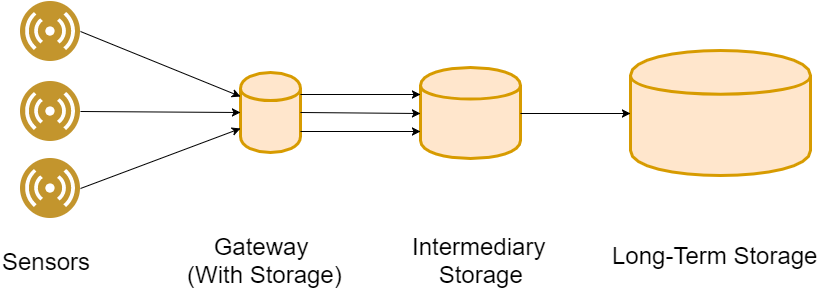
\includegraphics[width=\textwidth]{figures/pipeline.png}\\
\caption{Pipeline architecture}
\label{pipeline}
\end{figure}
The following section provides details on the design and implementation of the proposed IoT data delivery pipeline. 

In the context of a smart grid it is common to have a setup in which sensors are not directly connected to a data center to deliver the generated sensor data but connected to a gateway, that is close to the site of where the sensors are deployed. Also the gateway can then be connected to another intermediary hop, forming a so called "pipeline" to deliver the data to the data center. In such a scenario a sensor will send its measurements to the first gateway of the pipeline. The gateway will receive the message, maybe perform transformations to the data like aggregation, and forward the measurements to the next intermediary node in the pipeline. The intermediary node might also transform the data and forward it to the next hop. This process will repeat until the endpoint of the pipeline, the data center, will be reached. 

For that reason an implementation for such a pipeline has to be applicable not only to be run in data center but also on devices with limited resources available. This generates requirements like, being able to run on limited resources, as well as also performing well on limited resources. More over limitations in bandwidth, of the links between the different gateways in the pipeline should be considered.
Figure \ref{pipeline} provides an overview on the given pipeline architecture. Moreover should the gateways and intermediary nodes provide a suitable amount of storage to be able to deal with outages of a subset of the nodes in the smart grid. This should prevent data loss in a big scale and ensure that the pipeline and especially the smart grid, can remain operational in case of any partial outages. For that purpose also different and limited storage capabilities have to be taken into account when designing and choosing the database for the different types of nodes throughout the pipeline. The following will therefore provide a description of the technologies that are used for the first prototype implementation to meet all the different requirements and provide a description on how the components are implemented.


\subsection{gRPC}
GRPC is an open source remote procedure call(RPC) framework, that is built on top of HTTP2 connections and using Google Protocol Buffers for serializing the data that is transmitted and as interface description language. It provides an abstraction of the interfaces that have to be implemented and enables users to use different programming languages to implement their services. Many popular programming languages are supported, like Python, Java and C++. It also supports different platforms and can run in different environments, including data centers but also smaller and mobile devices. In addition to the afore mentioned gRPC provides support for bi-directional and client streaming RPCs and promises high performance. All the mentioned points make gRPC a suitable framework to choose for our pipeline implementation, since it promises to provide high performance in terms of throughput as well as latency, ease of use to the support of many different programming languages and the use of Google protocol buffers. The following section describes Google protocol buffers in general, how the developed message protocol for the pipeline implementation looks like and how the services are defined \cite{grpc}.
\subsubsection{Google Protocol Buffers}
 Google Protocol Buffers are a language and platform independent method to serialize structured data and generate the needed code for many different programming languages. It supports Python, Java, C++ and others. The message format has to be defined in a .proto file following the Protocol Buffer Language. After the .proto file is created, the code in the desired language can be generated. Google Protocol Buffers promise to be fast and small in size, and compared to XML offer 20 to 100 times faster serialization and 3 to 10 times less size \cite{protobuf}.
 The following will provide an overview on how the developed message format for the given task looks like.

\subsubsection{Message Format}
In order to be able to make use of the sensory data for the services needed to be deveolped for the given task, a message format had to be designed. The available parameters generated by each sensor in the smart grid was given. These parameters are: 
\begin{itemize}
\item Meter ID, an unique ID of a sensor
\item Metric ID, an unique ID to define the metric of a value
\item Timestamp, a timestamp with the time the sensor value got created
\item Value, a sensor measurement value
\end{itemize}
To reflect the parameters generated by the sensors, the measurement message format is created in the .proto file as follows:
\begin{lstlisting}
message measurement_message {
  string meter_id = 1;
  string metric_id = 2;
  int64 timestamp = 3;
  double value = 4;
}
\end{lstlisting}
With that all the needed parameters generated by a sensor are reflected in our message format. In addition to that two further parameters are needed, taking the proposed Provenance API into account. The additional parameters are:
\begin{itemize}
\item Provenance ID, an unique ID to identify a specific provenance datapoint
\item Context Parameters, a string containing all enabled context parameters 
\end{itemize}
To reflect these parameters as well, the following message format was created:
\begin{lstlisting}
message Grid_data {
  measurement_message measurement = 1;
  string prov_id = 2;
  string context = 3;
}
\end{lstlisting}
So the Grid\_data message contains a message following the measurement\_message format and the needed parameters for the Provenance API. Note that each field in the message is optional by default, so not every field in a message have to set.
In addition to the messages defined, a reply message was defined, that only contains a response code that follows common HTTP Status codes.
\begin{lstlisting}
message reply {
  string response_code=1;
}
\end{lstlisting}
With the defined messages, all the needed parameters originating from the sensors and the parameters of the Provenance API can be reflected.

\subsubsection{gRPC Service Definition}
In addition to the message format, a service definition, so an interface for the pipeline components has to be defined. To provide a preferably adaptable interface for all types of gateways between the sensors and the Long-Term Storage, one service was defined as follows.
\begin{lstlisting}
service gateway {
  rpc push_data(stream Grid_data) returns (reply) {}
}
\end{lstlisting}
With that the gateway service is defined, which exposes one RPC called push\_data. The push\_data RPC expects an input stream of messages of type Grid\_data and responds with a message with type reply. This means that the service is receiving a stream of messages, so several messages of type Grid\_data at once. The decision to implement it in this way was made due to the fact that otherwise the reply would have to be sent after each received message, which in return would increase network overhead. The benefit of using gRPC for the definition of the message format and the interface is that with the defined .proto file, the needed serialization code and code stubs to implement the RPC service can be generated in the programming language one desires. It was also the basis for the sensor data emulator described in the following section.

\subsubsection{Sensor data emulator}
Based on the already described message format and the service definition, we were provided with an emulator to simulate the generation of sensory data. It was used to simulate the sensors in a pipeline scenario.

\subsection{Local Storage}
As already mentioned, a way to store measurement messages on each node of the pipeline locally, is needed. The chosen database has to be able to run on all the different types of nodes, so it has to be able to run on smaller and less powerful gateway nodes and more performance offering nodes as small servers or in data centers. More over it has to provide a high write performance to be able to deal with a high load of receiving messages and therefore write operations. It also has to be scalable, lightweight and quick to respond. In addition to that and to be able to deal with the use case specific problem of outages in a smart grid, the database also has to offer persistent storage.  
\subsubsection{Redis}
Taking into account the data model of a measurement message, the decision was made to use a key-value storage database. In addition to that all the listed requirements have to be met, and especially keeping in mind the need for a database coping with different hardware configurations, the key-value in-memory database Redis was finalized as database to be used.
Redis meets all the requirements such as high performance on write operations. Even though it is an in-memory database it also provides the possibility of being persistent. Snapshots and write operation logs, can be used to provide persistence \cite{redis}. 

The following section will provide an overview on the implementation and explains the most important parts of it in detail.
\subsection{Implementation} \label{pipeline_implementation}

\begin{figure}[h]
\centering
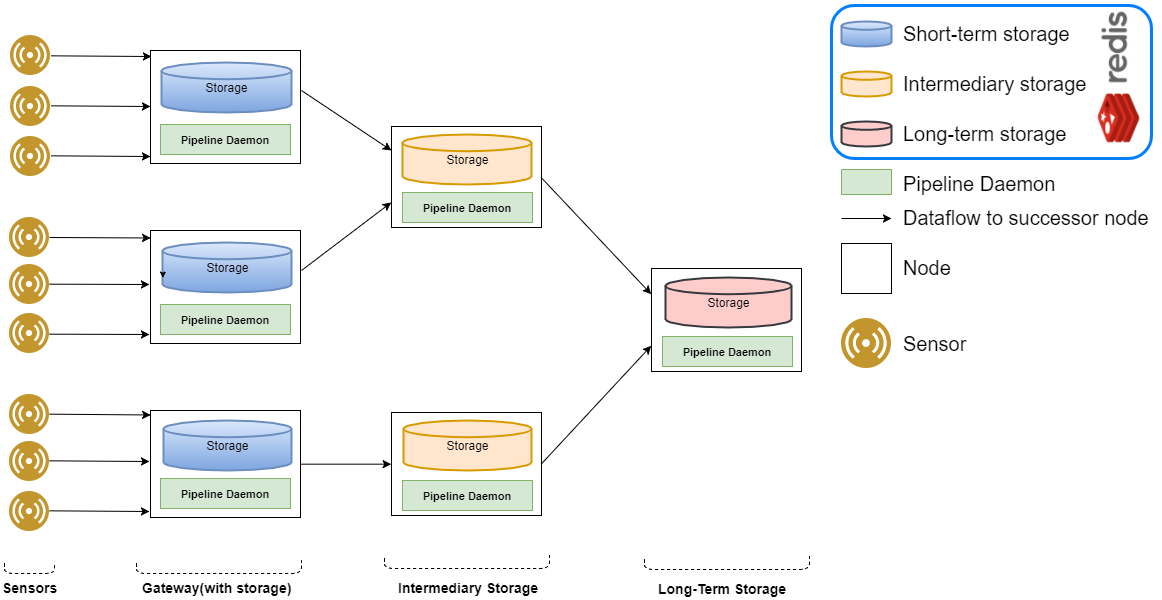
\includegraphics[width=\linewidth]{figures/pipelinearchitecture.png}\\
\caption{Pipeline architecture}
\label{pipeline_arch}
\end{figure}
In this section a detailed description and explanation of the pipeline implementation is presented. The pipeline is implemented in the programming language Java. For the build management, Apache Maven is used. The Java project is organized as follows. The code for the pipeline component resides in the PipelineComponent class. In addition to that the PipelineInterfaces.proto file provides the already described service and message definitions used to generate the serialization and service stub code. 

First of all, the system architecture is visualized in figure \ref{pipeline_arch}. One node in the pipeline consists of a database to provide local storage and a Pipeline Daemon.
The Pipeline Daemon is used to implement the already described service gateway.

\subsubsection{Pipeline Daemon}
The generated gRPC code was used to implement the gateway service and its RPC push\_data. The different types of nodes, that can be part of the pipeline, can be created when starting a component, by the use of different run configurations. A Pipeline Daemon can either be run as a gateway or as an endpoint. For that purpose a set of configuration parameters are provided. The following parameters are available:
\begin{itemize}
\item port, the port used by the server of this Daemon
\item port\_next, the port of the next hop in the pipeline
\item host\_next, the hostname or IP of the next hop in the pipeline
\item location, a label for the current physical location of the node
\item storageTime, an integer value representing the time messages are stored in seconds
\item propertiesfile, specifying the path to the Provenance Daemons properties file 
\item no\_prov, flag that can be set to turn of the collection of provenance data and the use of the provenance system
\end{itemize}
If the parameters host\_next and port\_next are set, the Pipeline Daemon is recognized as a gateway. On the other hand if these parameters would not have been set, the Pipeline Daemon is recognized as endpoint of the pipeline, since there is no successor. In addition to implementing the service gateway, the Pipeline Daemon implements a client, based on the push\_data interface definition, to be able to make use of the gateway services of other components in the pipeline. This is the case if the Pipeline Daemon is started as gateway. Then it has to be able to receive the messages from another clients and forward them to the next hop in the pipeline. 

The gateway service provides the push\_data service, as mentioned. The push\_data service is responsible of processing the messages a client sent. The client can send messages one by one, or send them as a stream of messages, so the client can send many messages at once. If the client sends a message and the push\_data service is called, it will process the message. The push\_data service is responsible for collecting the needed context information to feed to the Provenance Daemon and provide information, e.g. how many messages are received and sent per second. In case of receiving a stream of messages the push\_data service will cache the received messages and the generated context information. If the stream exceeds the number of 10 messages, the cached context information will be already forwarded to the Provenance Daemon and the measurement messages will be sent to the next hop, while still receiving the stream of messages. If the stream the client sends contains less then 10 messages, the push\_data service waits for the stream to be finished, before forwarding the context information to the Provenance Daemon and forwarding the messages to the next hop in the pipeline. This behavior was implemented due to the fact, that it is possible to use one single stream to send a large number of messages. If the Pipeline Daemon would wait until all messages arrived it is possible that additional delay is introduced and the latency increases. More over it would also result in irregular peak workload on the network, which is prevented when splitting up the incoming stream.   

Additionally there is the possibility that the no\_prov flag was set on startup of the Pipeline Daemon. In this case the push\_data service will not collect any context information. It will just cache and forward the measurement messages. 
The behavior of caching messages if the stream exceeds the number of 10 messages, remains the same. More over the provenance daemon will not be instantiated.

For the purpose of providing information like the number of messages per second to the developed user interface and to capture the health of the pipeline component daemon, additional methods are implemented by the push\_data service. A counter in combination with a timer is used to capture the number of messages. The advertisement of the values to the user interface is handled by the Provenance API. The node health is for one implicitly set when interacting with the provenance API, and for the other it is set by the use of a timer if the push\_data services is not interacting with the Provenance API.

\subsubsection{Local Storage}
For the use of the local storage, so the Redis database, a Redis client is implemented with the Pipeline Daemon. The push\_data service will, while processing the messages, save the measurement messages in the local Redis database. If the Provenance Daemon is active the Provenance IDs, that are received after the created context datapoints are handed to the Provenance Daemon, will be used as the keys for the measurement messages. This will also ensure, that in case of a failure the original messages can be retrieved from the local database and linked to the provenance entries in the Provenance DB. In contrast to that the current system time in nanoseconds is used if the no\_prov flag has been set. The measurement messages are saved as hashes, so with one key a whole measurement message can be saved.

The implementation of a Pipeline Daemon and the gateway service that is used for all different types of nodes, remains the same. From service implementation point of view it will only be differentiated between gateways and endpoints of the pipeline, so if messages will be forwarded to another hop in the pipeline or not. Only the amount of local storage provides a differentiation between different nodes. To be able to reflect this in the implementation, the storageTime configuration parameter is used. The parameter is used to simulate the different amount of storage available on the different machines that are part of the pipeline. A timer is used along with the specified time of the storageTime parameter so that after the timer expires the database will be flushed. With this it is ensured to reflect different storage capabilities with the Pipeline Daemon prototype implementation.







\section{Data Provenance Model}
\lstset{stringstyle=\color{black}}


\subsection{Existing Data Models}

\subsection{New Data Model}

We define a data point (DP) as a uniquely identifiable and addressable piece of data (i.e., a value) in the context of the smart grid. Examples for DPs in the context of smart grid includes sensor readings such as 3-phase electric currents, complex analytics results derived from sensor readings etc. The unique identifier is composed of three blocks.
\begin{itemize}
	\item Unique Identifier - A data point distinguishes itself specifically from other data flowing in the Data Provenance Model for smart grid  (e.g., bulk sensor readings that are of no further interest, ephemeral intermediary analytics results, etc.) in that it is addressable, i.e., it has an ID that is unique in the context of the smart grid. In order to ensure the uniqueness of the identifier, we came up with an identifier generation strategy, which generates a unique ten-byte identifier and ensures uniqueness across the system. Data point identifier comprised of:
		\begin{itemize}
			\item 3-byte node identifier - Guarantees its uniqueness across machines/nodes and processes.
			\item 4-byte value representing the seconds since the Unix epoch - Ensures uniqueness in relation to a single second.
			\item 3-byte counter - Provides uniqueness within a single second in a single process.
		\end{itemize}
		\subsection* {Properties} Our unique identifier mechanism along with its simplicity brought some other advantages and reduced the need to store machine/node identifier separately and also ease some time-based queries (e.g., sorting based on generation timestamp).
			\begin{itemize}				
				\item Example: 5a7b91370003c6badfb2
			\end{itemize}
	\item Input Data Points - A data point may be based on other data points that have contributed to its creation or modification. We refer to these related
data points as input data points(IDP). A data point's IDP is a list of unique identifiers of all those data points, which contributed to its creation or transformation. It also stores information about the contribution type.
	
	\begin{itemize}			
			\item Example: 
\begin{lstlisting}			
[{
    "average": [   // Contribution type
        "5a81c07800031ddaf123",
        "5a81c09300031d341fab"
    ]
}]		
\end{lstlisting}
	\end{itemize}
	\item Context - Specific context for provenance may vary for different IoT applications. We propose a data model for the context in typical IoT environments comprising the concepts of Agents, Execution Context, as well as Time and Location information. An Agent is an entity that creates and/or modifies data points (e.g., sensor, software agent, device, etc.). It is recursively defined in such a way that an agent can contain other agents (e.g., a device containing several sensors). This recursion allows for defining agents in a hierarchy and may be used as fine-grained as required. For instance, an agent hierarchy may span from the concept of a particular function in a software library running over a virtualization container on a particular device to a particular IoT network.
		
\begin{figure}[h]
\centering
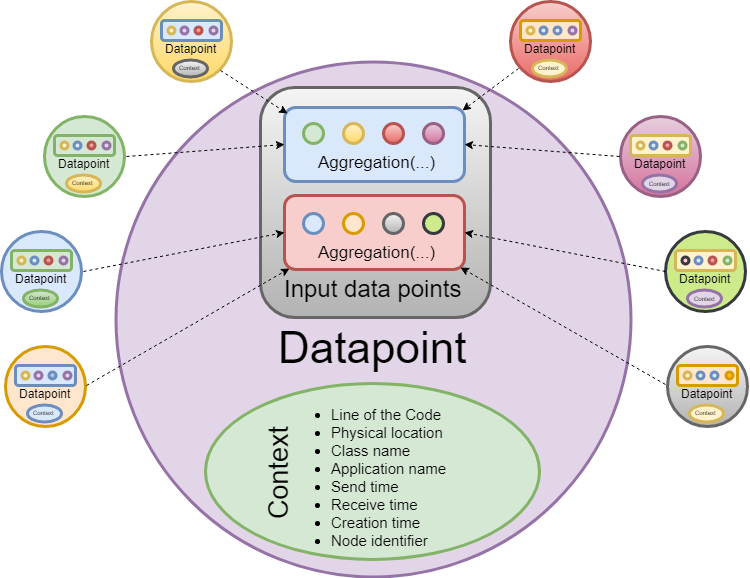
\includegraphics[width=\linewidth]{figures/dataModelforIDP.png}\\
\caption{Data Model}
\label{dataModel}
\end{figure}
\end{itemize}
TODO
\section{Provenance}

TODO
\section{Provenance Database}

Database is at the heart of every architecture especially when there a focus on the data. Choosing the right database goes a long way and the effect of this will be shown in each and every component of the architecture. In IoT domain where the data ingestion is huge and the data needs to query in real-time having a particular set of queries from where the user can query the dataset makes the decision more difficult.

In order to come up with the suitable database we underlying few basic factors which play an important role in finding the perfect match for the our system.

\paragraph*{Size of data to be stored:}
This factor considers amount of data stored and retrieved. So we choose the database keeping in mind the overall volume of data generated by the application at any given time and also the size of the data which is retrieved can handle efficiently.

\paragraph*{Speed and Scalability:}
This factor considers the speed of reading data from the database and writing data to the database. Some database focuses more on the read-heavy application, while others are designed to cope with the write-heavy operation on the application. This factor is important to our case as more data is writen to the database when adding new resources.

\paragraph*{Accessibility of data:}
Accessibility of data is important as the user of the system need to access the information as soon as possible it is stored for querying. The database needs to handle concurrent writes by numerous component in the architecture connected to the database. The effect of a huge load of writes should be minimum and there should be a mechanism in place which handles fault tolerance in the database. This will ensure all the provenance information is safe and is not lost forever.

\paragraph*{Data modeling:}
The structure is the core component in choosing the right database for the application. As the data from the sensors and the provenance information vary a lot. The data model is not specifically fixed in hard boundaries but can be capped under major categories. The database must be able to handle changes in the data model and adapt quickly.

\paragraph*{Safety and security of data:}
Storing information about the data from the sensor deployed on the ground capture various metrics which are confidential and contains information which is critical. In order to preserve the confidentiality and secrecy, the database must handle some level of security. The safety measures implemented by the database in case of any system crash or failure is quite a significant factor to keep in mind while choosing a database especially in our case where data lost means permanent loss of information.

\subsection{Apache Cassandra as Provenance Database}

After thoroughly considering a numerous number of databases from the pool we decided to use Apache Cassandra as the Provenance Database for our system.
Apache Cassandra is an open source, distributed, massively scalable NoSQL database. It is designed to handle large volumes of structured, semi-structured and unstructured data across multiple data centers, and it supports the cloud deployment. Cassandra offers capabilities like continuous availability, linear scalability and operational simplicity across many commodity servers with no single point of failure. Its powerful, dynamic data model is designed for maximum flexibility and fast response times. 

Apache Cassandra supports configured consistency levels to manage availability versus data accuracy for writes-heavy demand in IoT domain.  Data is compressed up to 80 percent without any performance overhead this can lead to storing more volume of data in less amount of space. 
Data is distributed across the cluster and there is no master node in the system so each node can service any request. The distributed architecture is perfect for disaster recovery, redundancy and failover as the data are different to create from the start.It can handle massive data sizes and scale out to large clusters. 

Apache Cassandra offering continuous availability, high scalability and performance, strong security, and operational simplicity. It has flexible data storage which easily accommodates the data in various formats and structure. Changes can be made dynamically to the data structure as per requirement.


Apache Cassandra outperformed other NoSQL database in the benchmark using YSCB and was also run on the sample dataset of our data model and performed fairly in term of writes. 
Apache Cassandra is the best choice for our scenario as it fulfills all the of providing a high write performance with a high load of receiving a message from a different component of the pipeline and the data is quickly available for the user to query. For IoT domain scenario, most of the nodes are distributed in numerous location so deployment of Apache Cassandra at different geographically distributed region could help in increasing the performance and also for faster retrieval of data.

\paragraph*{Apache Cassandra Query Language}
The Cassandra Query Language (CQL) allows you to query Cassandra using queries similar to SQL.CQL commands include data definition queries (e.g., create table), data manipulation queries (e.g., insert and select for rows), and basic authentication queries to create database users and grant them permissions.This fulfills the requirement of the user querying the provenance database for retrieval of provenance information.







\section{User Interface}

    Today most IS systems are based upon a Client-Server architecture, a three-tiered approach. The server performs the grunt of all operations where as the client side is more concerned with how to present the data. The processes that go on in these tiers can be represented by many more tiers, for instance a database tier can be added, where all data is stored can be represented by the diagram below. However it is important to note that more than one tier can be stored on one server, for instance both the web server and database servers each represent there own tiers in the diagram below, but in reality they could be seen as one.

    To  implement  a  web  application for Error detecting and monitoring system, client-server  architecture  is  required.  The  most  popular  client-server architectures  are  the  two-tier  and  the  three-tier architecture. The choice   of   architecture   affects   the   development   time   and   the   future   flexibility   and maintenance  of  the  application.  While  selecting the  architecture  most  suitable  for  an  application, many  factors  including  the complexity  of  the  application,  the  number  of  users and their geographical dispersion are considered. This system  is designed  based  on  a  traditional  three-tier  architecture  used  by  many  web  applications. Three-tier architecture  includes  a  presentation layer,  business  rules/  logic  layer, and the data layer (provenance database). The three-tier architecture is shown in Figure \ref{fig:architecture}.

    \begin{figure}
        \centering
        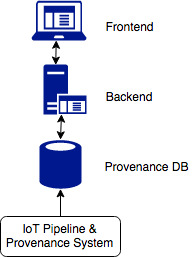
\includegraphics[width=0.4\textwidth]{figures/architecture.jpg}
        \caption{\label{fig:architecture}This is three-tier architecture.}
    \end{figure}

    Three-tier architecture gives an enhanced security, through the implementation of several layers, enhances the data security on a service-by-service. As client do not interact with the database directly, it provides less risk and conflicts with unauthorized data. Also it improves the data integrity as data corruption through client application can be eliminated as the data is passed in the middle tier for database updates ensures its validity. Due to distributed deployment of application servers, scalability of the system is enhances since a separate connection from each client is not required whereas connections from few applications servers are sufficient.
    \newline
    \newline
    The three-tier architecture is generally used when an effective   distributed client/server design is needed that provides
    \begin{itemize}
        \item increased performance
        \item flexibility
        \item maintainability
        \item re-usability and
        \item scalability
    \end{itemize}

    This  model hides  the  complexity  of  distributed  processing  from  the  user.  These features   have   made   the   three-tier   architecture   a   popular choice over the two-tier architecture for Internet applications. The three layers are discussed below.
    \newline
    \newline
    The \textbf{Data layer} is  responsible  for  data  storage.  Primarily  this  tier  (layer)  consists of one or more relational databases and/or file systems.
    \newline
    \newline
    The \textbf{Business Rules/Logic layer} is the middleman between the presentation layer and  the  data  layer. This  middle  tier  was  introduced  to  overcome  the  deployment limitation (whenever
    the application logic changed the application had to be redistributed at  each  and  every  client)  in  the  two-tier  architecture.  The  middle  tier  provides  process
    management where business logic and rules are executed and can accommodate hundreds of  users.
    \newline
    \newline
    The \textbf{Presentation  Layer},  also  called  the Client  tier,  is responsible  for the presentation  of  data,  receiving  user  events,  and  controlling  the  user  interface.  The  user
    interaction with the system is entirely through this layer.
    \newline
    \newline
    The three-tier architecture for Smart-grid IoT provenance system's Error detection use-case. The data layer in this architecture comprises of Provenance Database of the system, in this case here we have used Cassandra. The logic layer/business layer is defined by Java's Spring boot framework and provides REST component to the Presentation layer and the messages are communicated by JSON. And the Presentation layer where the data is represented to the end-user is developed in Node.js Express framework with Jade view template engine.
%backend
%frontend
\section{Testing and Deployment}
While our planning phase in the first third of the project, we decided to assign responsibilities to team members for different parts of the implementation.
This leads to an independent implementation workflow for every component with the need to put them all together at some time - not only for a final deployment, but also for development of the dependent components ( for instance the pipeline component that use the Provenance API).
To realize a fast development of depenent parts and produce runnable artifacts at any time (as it is usual for a Scrum schedule), we decided to implement a Continuous Integration Workflow based on the commits that was made to the respective Repositories. Each commit was automatically tested (at least whether it is buildable) and, if it was desired, deployed to a Docker or Maven Repository. The current build state of each branch was evaluated immediately after a push so that the code health could be checked by erveryone at any time.
On this way, other parts of the project could include the artifacts by using explicit version tags or \emph{LATEST}-version of the repositories. In the first part of this section, we will describe in detail, how we implemented our CI workflow. In the second part we describe how we used these artifacts for a deployment on AWS\footnote{We used the aws deployment also for our benchmarks (\ref{}).} and which additional adjustments were necessary to get a larger deployment with individual sensor workloads.

\subsection{Continuous Integration \& Delivery}

\paragraph*{Travis CI}
%For every component of our provenance system we created a Github Repository and registered 
%\begin{itemize}
%	\item Pipeline Component \footnote{\url{https://github.com/Krymnos/IDP}}
%	\item Backend\footnote{\url{https://github.com/Krymnos/IDP-backend}}
%	\item Frontend\footnote{\url{https://github.com/Krymnos/IDP-frontend}}
%	\item Provenance API\footnote{\url{https://github.com/Krymnos/Provenance-System-for-IoT}}
%\end{itemize}
%

\begin{figure}[h!]
	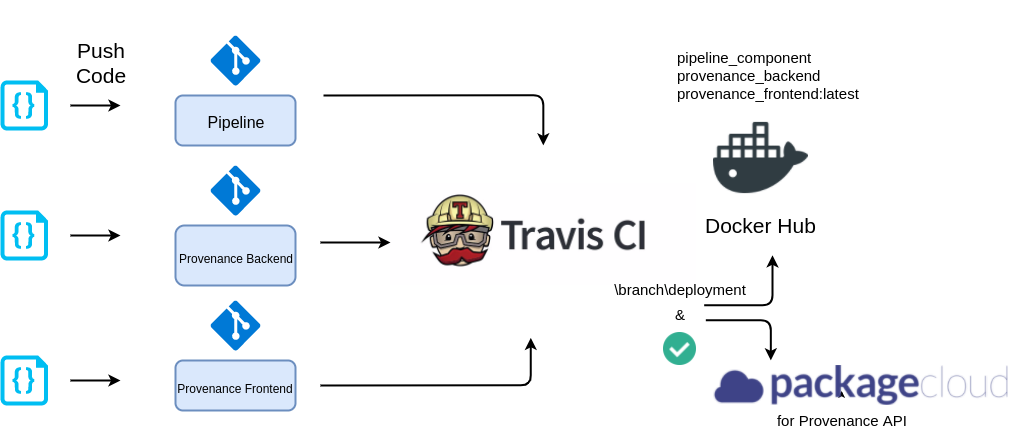
\includegraphics[width=\textwidth]{figures/deployment.png}
	\caption{Deployment Pipeline}
	\label{fig:deployment}
\end{figure}


We used Travis CI\footnote{\url{https://travis-ci.org/Krymnos/IDP}} as Continuous Integration Solution that is free for Open-Source Projects. Travis builds were triggered on changes for every branch of the repository that contains a valid \emph{travis.yaml}.
The testing configuration was set inside of the \emph{travis.yaml} that was present in each repository. Some components needed additional configuration to get builds and tests running. For instance, the Pipeline Component needs the protobuf executables to generate the communication interfaces during a build. After a the compilation is finished, the unit tests of the Pipeline requires a running \emph{Redis}-Database as local storage. All these configurations could be made by the \texttt{before-script} and \texttt{before-install} sections inside the \texttt{travis.yaml} by using the built-in services of travis\footnote{\url{https://docs.travis-ci.com/user/database-setup/}}. As an example, the travis.yaml for the pipeline component can be found in the appendix \ref{lst:pipelineyaml}.
At the same file a \emph{deployment}-section was defined and only executed if the branchname is equal to "deployment". For the components that are delivered as docker builds, the respective docker deployment script was executed \ref{lst:dockerdeploy}, for the Provenance API that is included by the Pipeline Component, the artifacts was pushed to our Maven Repository\footnote{\url{https://packagecloud.io/gerritja/IDP}}. The docker deployment script pushed the docker images to \emph{Docker Hub}-Repository of our project\footnote{\url{https://hub.docker.com/r/cloudproto/}}.

\paragraph*{Docker Images}
We decided to use Docker for the deployment of our components because a docker container runs platform independent, isolated, lightweight and can be interconnect with other services in a very simple way \footnote{\url{https://docs.docker.com/engine/docker-overview/\#docker-engine}}. The Docker engine (in combination wirh docker-compose or Docker Swarm) also supports a good functionality to bring a deployment to a large scale. That suites well to our plans for a fast iterative development and the possibility to test our system on different Topologies.

To deploy our components as Docker images, we added a \emph{Dockerfile} to the Sensor, Pipeline, Backend and Frontend components. A Dockerfile\footnote{\url{https://docs.docker.com/engine/reference/builder/}} contains the instuction that are executed during a build of an image. As well it's defined in a Dockerfile which commands has to be executed on an instantiation of a Container. For the Pipeline Component, for instance, we specified that every instance has a Redis Database running that was started inside the docker container as a local daemon.

To make the Docker Container configurable, we introduced environment variables for the Provenance API and further settings. Also delaying the runtime of the Pipeline Component by setting \texttt{STARTUP\_DELAY}) is possible because we noticed that we had undesired failures at startup because depedent components were not available due a longer instantiaion phase\footnote{for instance, the cassandra database takes usually more time to be available than a lightweight pipeline component}. As an example, the Dockerfile for the pipeline component can be found in the appendix (\ref{lst:pipelinedockerfile}).

\paragraph*{Setup Topologies with docker-compose Files} 
For manual testing of our System and running benchmarks (\ref{chap:Benchmarks}), we defined the individual components and the connection between each other inside a compose file for Docker \footnote{\url{https://docs.docker.com/compose/compose-file}}. The compose files could be therefore used as specification for a deployment with Docker or Docker Swarm.

A simple example that defines a simple pipeline with a workload generator, a gateway and an endpoint can be found in the appendix (\ref{lst:simpletopology}).
The topology can be started on any machine that has Docker installed and a docker-compose and/or docker swarm extension.

\begin{itemize}
	\item command for docker swarm:\texttt{docker stack deploy -f <composefile> <stackname> }
	\item command for docker-compose:\texttt{docker-compose -f <composefile> up} 
\end{itemize}


\subsection{Docker Swarm on AWS}
Due to the machine independability of docker containers we're able to deploy our topology locally but also along distributed machines.
As \emph{docker-compose} is sufficient for a local deployment on one node, \emph{Docker Swarm} is used to distribute the orchestration of the components over multiple machines which are organized within a cluster and running on \emph{swarm mode} \footnote{\url{https://docs.docker.com/engine/swarm/key-concepts/}}.

To setup such a cluster on AWS we used a predefined Cluster template for \emph{AWS Cloud Formation}\footnote{\url{https://editions-us-east-1.s3.amazonaws.com/aws/stable/Docker.tmpl}} that is provisioned by Docker \footnote{\url{https://docs.docker.com/docker-for-aws}}. A detailed readme, how a topology can be deployed is available on the IDP repository on \texttt{deployment/howto.md}\footnote{\url{https://github.com/Krymnos/IDP/blob/master/deployment/howto.md}}

\subsubsection*{Scaling of Sensors/Workload}
For our project we got circa 6 GB of real sensor data with measurements of a power grid. The data contains folders for every day in a year. Each folder contains usually 10 data items (csv files), each is representing a sensor. We wanted to be able to test more than 10 sensors in our deployment.

\paragraph*{data preparation}
We modified the origin strucure of the sensor data in a way that one folder contains all files to simulate many more sensors for only one day.
The workload generator that sends the data to our pipeline components determines a sensor id by the filename (e.g. \texttt{31400010000000000.csv}). We had to rename the files due to the issue of having many duplicate filenames. We numbered the files consecutively to get increasing sensor ids (from 31400010000000000 to 31400010000003473) so that we're able to simulate up to 3474 unique sensors\footnote{\url{https://s3.console.aws.amazon.com/s3/buckets/provenancesensordata/data/oneday} note: the access to the sensordata is restricted due to privacy reasons}.

\paragraph*{data inclusion}
To have the ability to run a sensor container completely without external sensor data, we stored a small dataset (few megabytes) inside the sensor container-image.
For our plans to scale sensors with unqique sensor data it was obviously not an option to put 6 GB into a docker image. Also the creation of thousands of sensor images (with few megabytes for a unique sensor) makes no sense.
Therefore, we stored the sensor data to a \emph{Amazon S3} Bucket and implemented a docker image for the sensor that has the skill to mount bucket inside the local filesystem of the container\footnote{We forked an existing base image to add this functionality \url{https://github.com/serioja90/docker-goofys}}. An example that can be used inside a docker compose file can be found in the appendix \ref{sensors3}.

This approach worked fine for a local deployment on one node by using \emph{docker-compose}. Unfortunately, we had to realize, that this image doesn't work on \emph{Docker Swarm}, because the priviliged execution of the docker container is mandatory to mount the S3 Bucket inside. The priviliged mode is supported by \emph{docker-compose} but not by \emph{Docker Swarm}\footnote{a discussion/open issue about that can be found here: https://github.com/moby/moby/issues/24862}.
To get a working access to the S3 bucket, we defined an external \emph{docker volume}\footnote{\url{https://docs.docker.com/storage/volumes}} in the compose file in combination with a docker plugin that links the S3 bucket with the docker volume \footnote{https://hub.docker.com/r/rexray/s3fs}.

\paragraph*{scalable sensor groups}
At this point, we were able to mount the complete sensor data on a efficient way. We still had the problem, that a definition of unique sensors was only possible by adding a service entry for every single sensor to the compose file, because the sensor was explicitely expecting the datapath to the measurement file.
Docker provides a scale command \footnote{\url{https://docs.docker.com/compose/reference/scale/}} that can be used to scale up services of indentical instances. To define sensor groups of unique sensor by using this command we implemented another service for sensor-id coordination. This service implements a simple counter that gives the current id as an response of a REST-Request and increments it.
We modified the sensor code in a way, that a sensor calls the REST endpoint of the coordinator and adds the received id to the basepath of the sensordata folder on the mounted data\footnote{The implementation of the coordinator and the modifications in the sensor implementation can be found here: \url{https://gitlab.tubit.tu-berlin.de/gerrit.janssen/smemu}}. 

The appendix contains a simple example of mounting the S3 bucket and the id coordinator approach\ref{lst:sensorsscale}


\subsubsection*{Deployment of the complete stack}
We created different versions of compose files with different Topologies and all components. The files can be found in the IDP-Repository at: \texttt{compose-files}\footnote{https://github.com/Krymnos/IDP/tree/master/compose\_files}. In this folder exists also a readme that describes, how to instatiate a topology locally  with \emph{docker-compose}\footnote{ Some compose files containing special constraints for aws, for instance to schedule nodes in different availability zones.}.

Figure \ref{fig:finaldeployment} shows a the general scheme for a deployment on AWS.

\begin{figure}[h!]
	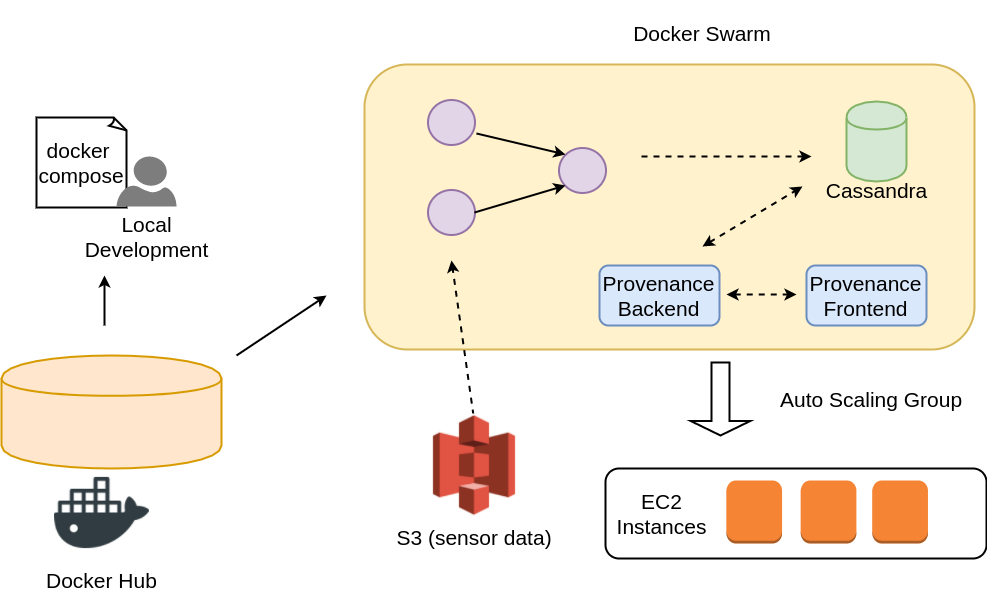
\includegraphics[width=\textwidth]{figures/deployment2.png}
	\caption{deployment scheme of the complete stack on AWS}
	\label{fig:finaldeployment}
\end{figure}
\chapter{Benchmarks}

In this chapter we describe the Benchmarks we performed to evaluate our system. 
The goals we had set beforehand are described in the Motivation section. 
Then the implementation of each Benchmark, their results and our evaluation are discussed separately.

\section{Motivation}

Based on the use-case described in the first chapter, we decided to evaluate our system firstly by looking at the overhead it adds to the bare pipeline implementation. 
Since this is one of the major concerns for users that worry about fixed hardware limitations of their system.

We distinguish two dimensions of overhead:

\begin{itemize}
  \item \textbf{Latency:} The time it takes for sensor value messages to be propagated through the pipeline.
	\begin{itemize}
	  \item Pipeline Latency: Difference in time between receiving a message at the first gateway and receiving it at the last gateway.
	  \item Node Latency: Difference in time between receiving and relaying a message from one node.
	  \item Channel Latency: Difference in time between sending and receiving a message in between two neighboring nodes.
	  \item measured in Milliseconds
	\end{itemize}
  \item \textbf{Data Volume:} The amount of data that is send along the network.
	\begin{itemize}
	  \item Recorded as traffic going \textbf{in} to each gateway and \textbf{out} of each one.
	  \item measured in KB/s
	\end{itemize}
\end{itemize}

Looking at failure scenarios had the goal to evaluate the functionality of our system, especially in regard to the time it takes to detect failures.
This was again motivated by our use case, where detecting failures in near real time was one the major goals for the grid administrators. 

\vspace{3mm}

When designing our benchmarks, we mainly made decisions based on the following assumptions we had about our systems at that point: 

\begin{itemize}
  \item The end user should receive notifications in near real time, i.e. within 10 seconds.
  \item Increasing the number of recorded context parameters will increase latencies slightly.
  \item Increasing the number of recorded context parameters will increase the data volume.
  \item Using the provenance system will increase data volume by a factor of 2 or more, over the bare pipeline implementation.
  \item There will be an ideal setting for the buffer capacity that is dependent on the remaining configuration.
  \item The results of our benchmarks will only give us qualitative indications of how the system will perform on an actual smart grid.
\end{itemize}


\section{Data Overhead}
Data Overhead is besides the latency one of the most important metrics especially for a geo-distributed system like a smart grid due to usually strong bandwidth limitations. Therefore it's very important to know which additional "message costs" are related to the use of our provenance system.

We performed several experiments with different provenance configurations as well experiments completely without provenance to determine how big the impact for the use of the provenance system is. We wanted also to determine which setting has more impact of the overhead and which has less to give a recommendation on a possible setup dependent on available bandwidth.
We did the benchmarks for different topologies that stand for usual patterns that can be found in real topologies. For each topology we will describe our assumptions and then evaluate the results of that.

\subsection{Test Setup}
To run the equal testconfiguration on every topology, we wrote a script\footnote{The script and the raw data of the measurments are available in the repository at \texttt{/benchmarks/overhead/benchmark.sh} and \texttt{/benchmarks/overhead/eval}} that goes through the steps shown in figure \ref{fig:benchmark}.
The benchmark script runs a 120 seconds long benchmark run on each topology with all combinations of the following configurations:

\begin{itemize}
\item metrics configuration :

We executed runs with full provenance (\texttt{meterid,metricid,loc,line,class,app,ctime,stime,rtime}) and made runs with each individual metric together with \texttt{ctime}, because this metric is mandatory for the correct functioning of the system.

\item buffer sizes : \texttt{1,5,10}
\end{itemize}

\begin{figure}[H]
	\center
	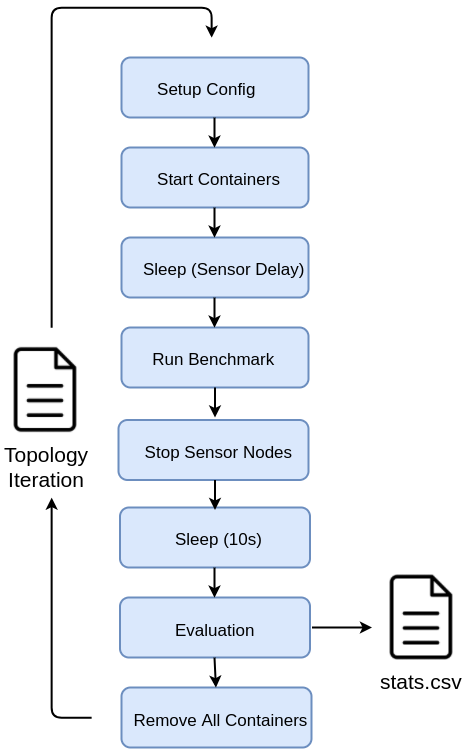
\includegraphics[width=0.5\textwidth]{figures/dataoverheadsetup.png}
	\caption{Benchmark Procedure}
	\label{fig:benchmark}
\end{figure}

The benchmark runs this combinations for each topology file that is defined inside the script. On the first step the respective metrics and buffer configurations are replaced in the compose file that contains the topology.
On the next step, the containers are started by \emph{docker-compose}. In the script is a fixed startup-delay for the sensors defined. We inserted this to ensure that all containers are running at the beginning of the benchmark runtime. On the "Run Benchmark" step, the script waits until the defined benchmark time of 120 seconds has expired. Then only the workload generator nodes are switched of. Another waiting time (10 seconds) is used to ensure that the sensor nodes are terminated and no pending messages are on the pipeline. Then the \emph{docker stats}\footnote{\url{https://docs.docker.com/engine/reference/commandline/stats/}} command is executed to get the \texttt{Net I/O} metrics for each container node. In addition to the docker stats, all local storages of the pipeline nodes are queried to get the number of messages that passed through the nodes. The retrieved stats are stored to a csv file that is created at the beginning of the script.
After "Evaluation" all containers are stopped and removed to guarantee that no run is influenced by an preceding run (e.g. restart of already "used" containers).

The fields of the measurements are:

\begin{itemize}
\item TOPOLOGY - the topology file that was used for the run
\item PROV\_METRICS - provenance metrics that was inserted to the config
\item BUFFER\_CAPACITY - provenance buffer config
\item COMPONENT - component of the pipeline
\item NET\_IN - NET\_IN stat from docker stats
\item NET\_IN\_TYPE - format of the NET\_IN value (B,kB,MB) 
\item NET\_OUT - NET\_OUT stat from docker stats
\item NET\_OUT\_TYPE - format of the NET\_OUT value (B,kB,MB) 
\item MSG\_NUMBER - number of messages that passed the component
\item NORMALIZED\_MSG\_SIZE\_IN - NET\_IN divided by MSG\_NUMBER
\item NORMALIZED\_MSG\_SIZE\_OUT - NET\_OUT divided by MSG\_NUMBER
\item NORMALIZED\_MSG\_SIZE\_TYPE - format (B,kb,MB)
\item BENCHMARK\_RUNTIME - runtime in seconds for the benchmark
\end{itemize}

\subsection{Test Cases}
\paragraph*{Single-Node Topology}
The purpose of the Single-Node Topology is to get the pure overhead that is produced only for one data item without any relaying of messages to other pipeline components.

\begin{figure}[H]
	\center
	
\includegraphics[width=0.3\textwidth]{figures/dataoverheadtopolabeled0.png}
	\caption{One-Node Topology}
	\label{fig:onetodetopology}
\end{figure}

We evaluated the proportion of the respective metrics by running each metric in a different run and divided the network output by the number of messages that was received by the endpoint. Because the "ctime" metric is a mandatory metric for every run, we substracted the run where only "ctime" was measured from all other runs. "ctime + base" is the run where only ctime was chosen as a metric. Using the network traffic to measure the impact of a metric shows not the real size of a single message. In this measurements are also the communication traffic of the whole system included (e.g. communication between node and cassandra db or traffic between node and docker). Even if the sizes are not the real message sizes, the diagram shows nevertheless the impact to the network traffic by choosing different metrics compared to the no-provenance case.

\begin{figure}[H]
	\center
	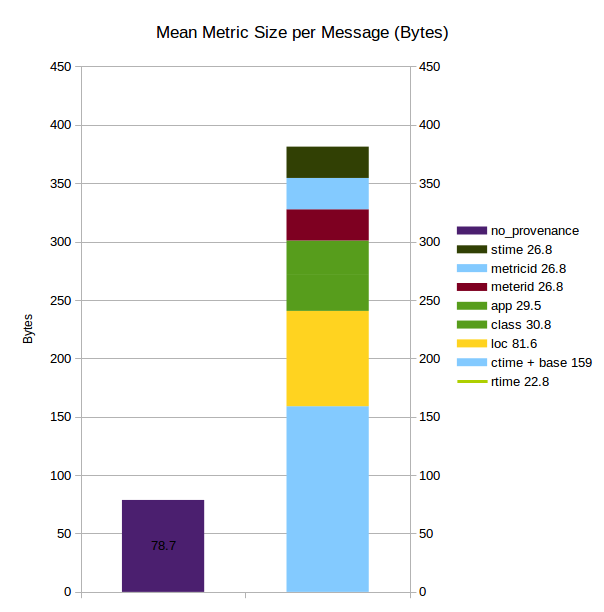
\includegraphics[width=0.7\textwidth]{figures/overheaddiagram1.png}
	\caption{Size Distribution for Metrics per Message}
	\label{fig:metricsdistribution}
\end{figure}

To determine the message size of the measurement, we  used  "NORMALIZED\_MSG\_SIZE\_IN" stats of the endpoint for the "no\_provenance" case.

The diagramm \ref{fig:metricsdistribution} shows, that the basic metrics and the location ("loc") are the largest parts of the message. The whole traffic is approximately 5 times bigger when the provenance system is used compared to the non-provenance case.

\begin{figure}[H]
	\center
	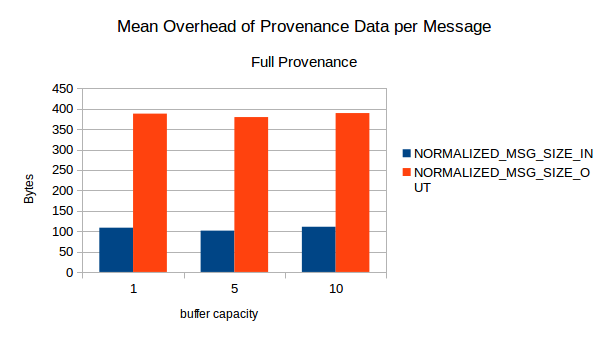
\includegraphics[width=\textwidth]{figures/overheaddiagram2.png}
	\caption{Different Buffer Sizes (Topology 0)}
	\label{fig:buffersizes}
\end{figure}

By using different buffersizes (1,5,10) no improvement can be observed on diagram \ref{fig:buffersizes}. This option may not improve the used bandwidth due to already existing buffer mechanisms in the the used technologies for the system\footnote{for example GRPC}.

\paragraph*{Two-Node Topology}
The purpose if running the Two-Node topolotcy is to evaluate how much the overhead grows due to an enrichment of the provenance data. This topology consists of one sensor and two pipeline nodes (Gateway, Endpoint) which also produced provenance data.

\begin{figure}[H]
	\center
	
\includegraphics[width=0.5\textwidth]{figures/dataoverheadtopolabeled1.png}
	\caption{Two-Node Topology}
	\label{fig:topo1}
\end{figure}

\begin{figure}[H]
	\center
	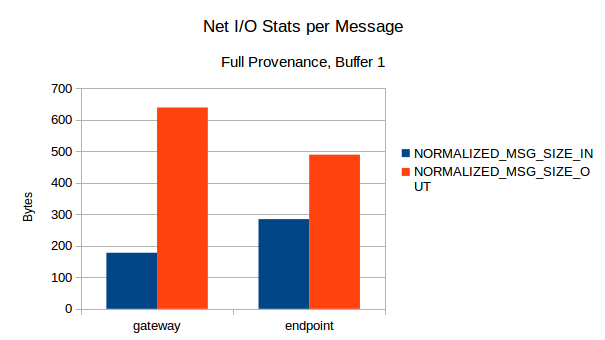
\includegraphics[width=\textwidth]{figures/overheaddiagram3.png}
	\caption{Mean Net I/O per Message (Topology 1)}
	\label{fig:topo1meanpermsg}
\end{figure}

\begin{figure}[H]
	\center
	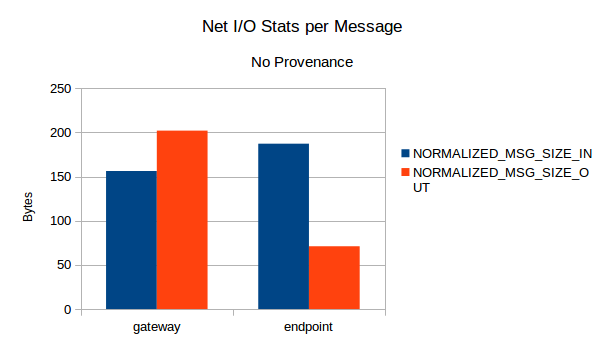
\includegraphics[width=\textwidth]{figures/overheaddiagram7.png}
	\caption{Absolute Net I/O for 7480 Messages (Topology 1)}
	\label{fig:topo1absolutenoprov}
\end{figure}

The diagram \ref{fig:topo1meanpermsg} shows, that the per message size of the gateway node is approximately 100 bytes larger than for the endpoint. That suites well to our measurement in diagram \ref{fig:buffersizes}\footnote{The NORMALIZED\_MSG\_SIZE\_IN in \ref{fig:buffersizes} is around 100 Bytes large. This value can be interpreted as the data size of a single smart grid measurement}. The difference between the NORMALIZED\_MSG\_SIZE\_IN value of gateway and endpoint can be interpreted as the overhead if we assume that the "IN" value of the gateway stands for a measurement of sensor without provenance. The overhead in that case would be therefore round 100 bytes of data that is pushed to the next node (besides the provenance data that is also being sent to the provenance db). Here as well, it needs to be taken into account that these values are not pure message overheads but an overall impact of the whole system. For example the I/O stats also contain the Heartbeat-Messages that were send between gateway and endpoint.

\begin{figure}[H]
	\center
	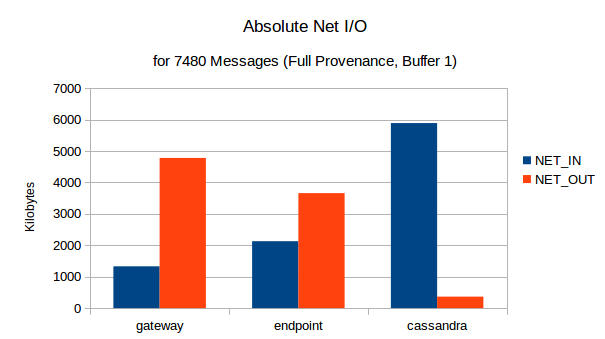
\includegraphics[width=\textwidth]{figures/overheaddiagram4.png}
	\caption{Absolute Net I/O for 7480 Messages (Topology 1)}
	\label{fig:topo1absoluteprov}
\end{figure}

\begin{figure}[H]
	\center
	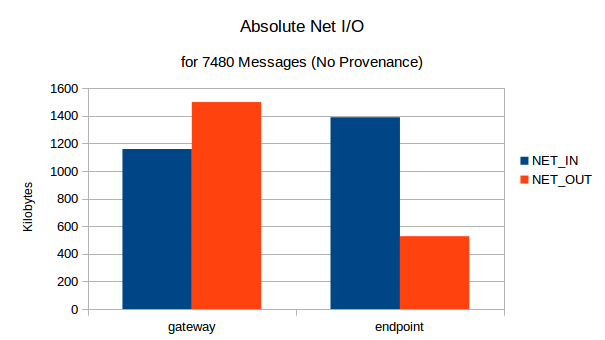
\includegraphics[width=\textwidth]{figures/overheaddiagram8.png}
	\caption{Absolute Net I/O for 7480 Messages (Topology 1)}
	\label{fig:topo1absolutewithouotprov}
\end{figure}

\paragraph*{Fork-Node Topology}
The Fork-Node topology consists of two sensor nodes which sends the measurements to two different gateways. These gateways (Gateway A,B) push the data to a common Gateway C. This Gateway sends the data further to another endpoint node.

\begin{figure}[H]
	\center
	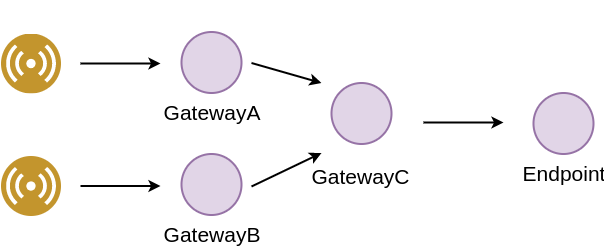
\includegraphics[width=0.7\textwidth]{figures/dataoverheadtopolabeled2.png}
	\caption{Fork-Node Topology}
	\label{fig:deployment}
\end{figure}

On this run of the benchmark we want answer the question whether the data overhead is growing on common gateways. As it can be observed in diagram \ref{fig:overhrad5} is the \texttt{NORMALIZED\_MSG\_SIZE\_IN} approximately 100 bytes larger than for gatewayA and gatewayB. This matches our observations in the previous benchmarks.
If we compare diagram \ref{fig:overhrad5} (Full Provenance) and  \ref{fig:overhead6}, we can observe that the Net I/O for gatewayC grows. It's difficult to get an explanation why the mean data is bigger. One would expect that there is no difference between different gateways at least for the non-provenance case.
However, we can assume that this growth of data traffic for gatewayC is not from the provenance system itself but from the pipeline implementation.

\begin{figure}[H]
	\center
	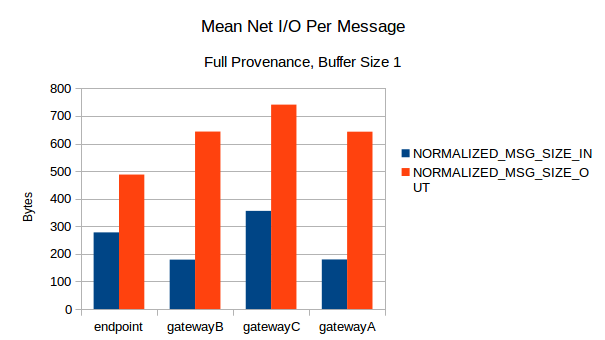
\includegraphics[width=\textwidth]{figures/overheaddiagram5.png}
	\caption{Mean Net I/O per Message (Topolgy 2)}
	\label{fig:overhrad5}
\end{figure}

\begin{figure}[H]
	\center
	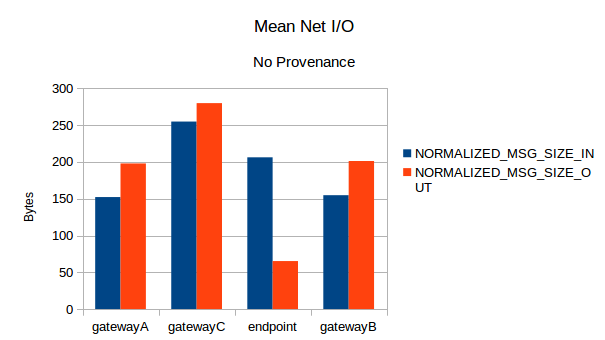
\includegraphics[width=\textwidth]{figures/overheaddiagram6.png}
	\caption{Mean Net I/O per Message (Topology 2)}
	\label{fig:overhead6}
\end{figure}

\subsection{Conclusion}
The data overhead was in our tests up to 5 times bigger than the real measurment data. This was also the case, when we used the minimal possible configuration for metrics \ref{fig:metricsdistribution} (2 times bigger).
This has to be take into account if this system ought to be used in bandwidth limited environments.
Nevertheless we can assume when we would have larger measurement messages, the provenance data will not be larger than in our measurements because the size of our metrics does not grow with larger measurements.
As already mentioned in the evaluation steps, the calculated mean values for the Net I/O are representing the full impact of the provenance system to the network interfaces and does not reflect the real size of messages.

\section{Latency Overhead}

TODO
\chapter{Benchmark}


\section{Failure Detection Benchmarks}

The purpose of this benchmarks is to find the following four types of failures,
    \begin{itemize}
        \item Node Failure
        \item Channel Link Failure
        \item Provenance Daemon Failure
        \item Pipeline Daemon Failure
    \end{itemize}

\section{Node Failure}

The purpose of this benchmark is to find the time taken to detect a node failure in the topology. Node failure is here meant to be the nodes that run the provenance daemon and pipeline daemon and not the sensors. If any of the nodes that are running the provenance API daemon and pipeline daemon are failed then messages sent via this nodes will be failed to reach the other nodes.

We need to measure the time taken metric for our provenance system to detect such a node failure. In our provenance database, heartbeat messages are sent by each node are stored in the HEARTBEAT table.

So the main tables that are needed to perform this benchmark are,
    \begin{itemize}
        \item Node
        \item HeartBeat
    \end{itemize}

\subsection{Method to generate a node failure}

Method to simulate a node failure is to kill the container(node) itself. Here the workload generator will introduce failures continuously at regular intervals by killing the docker container and restarting the docker container. This killing and restarting process will happen throughout the benchmark.

\subsection{Logic used to detect node failure}

We will be querying the Node table to get the list of nodes. Once we got the node id for a particular node, then we query the heartbeat table to get the rows with that id.

Once we get the rows, if heartbeat rows are available for the node then we can be sure that the node is active. We also need to perform an additional check to find out if the timestamp field is less than 30 seconds old. Because each node will be sending the heartbeat messages every 30 seconds and we need to be sure that the node is active currently. We will store the timestamp value each time in the benchmark and compare it next time with the previous value to find out if the heartbeat message is the latest one.

\section{Link Failure}

The purpose of this benchmark is to find the time taken to detect a channel link failure in the topology. Channel link failure is here meant to be physical link failure. If any of the channel links between the nodes that are running the provenance API daemon and pipeline daemon are failed then messages sent via this nodes will be failed to reach the other nodes.

We need to measure the time taken metric for our provenance system to detect such a failure. In our provenance database, heartbeat messages are sent by each node are stored in the HEARTBEAT table. Also to check if the neighbouring nodes are active and also to detect link failures, we also send messages to neighbours and each node will transmit those messages to the provenance database. 

So the main tables that are needed to perform this benchmark are,
    \begin{itemize}
        \item Node
        \item HeartBeat
    \end{itemize}

\subsection{Method to generate a link failure}

There are two ways to generate a link failure,
    \begin{itemize}
        \item During the deployment of the topology, 'host_next' parameter in the topology yaml file which is used to provide a virtual link between containers(nodes). We will be changing the name of this field to some random value and thus making the two containers unreachable. There-by simulating a link failure between nodes in the provenance system.
        \item Another method to simulate a link failure is to kill one container(node) itself. Because once the deployment is done and the topology is running in the provenance system, killing the container(node) is the only way to simulate the link failure in the docker environment.
    \end{itemize}

Here we have used the first method and during the deployment itself we provide a wrong connection between the nodes and we run the benchmark test to detect those failures.

\subsection{Logic used to detect link failure}

We will be querying the Node table to get the list of successor for each node. Once we got the successor for a particular node, then we query the heartbeat table to get the rows with the id of the successor node and also with its own id.

Once we get the rows, if heartbeat rows are available for the node and its neighbour then we can be sure that both the nodes are active.
The next check we need to perform is to find if the channel field in the heartbeat table row with the successor id contains the node id.
If the node id is present then we can conclude that channel link is also active. We also need to perform an additional check to find out if the channel field is less than 30 seconds old. Because each node will be sending the heartbeat messages every 30 seconds and we need to be sure that the channel is active currently.

\section{Pipeline Failure}

The purpose of this benchmark is to find the time taken to detect a pipeline daemon failure in the topology. Pipeline daemon failure is here meant to be process failure in a node that is running the pipeline API. If the process in a node that is running the pipeline API daemon are failed then heartbeat messages and provenance messages will not be processed in this node and sent to the database and also not sent to the neighbouring nodes in the topology.

We need to measure the time taken metric for our provenance system to detect such a failure. In our provenance database, heartbeat messages are sent by each node from the pipeline daemon and are stored in the HEARTBEAT table.

So the main tables that are needed to perform this benchmark are,
    \begin{itemize}
        \item Node
        \item HeartBeat
    \end{itemize}

\subsection{Method to generate a pipeline daemon failure}

Method to simulate a pipeline daemon failure is to kill the container(node) itself. This is similar to the Node failure detection benchmark we have done earlier. Here the workload generator will introduce failures continuously at regular intervals by killing the docker container and restarting the docker container. This killing and restarting process will happen throughout the benchmark.

\subsection{Logic used to detect pipeline daemon failure}

We will be querying the NODE table to get the list of nodes that are running the pipeline daemon. Once we got the node id for a particular node, then we query the heartbeat table to get the rows with that id. 
Once we get the rows, if heartbeat rows are available for the node then we can be sure that the pipeline daemon is active. We also need to perform an additional check to find out if the timestamp field is less than 30 seconds old. Because each pipeline daemon will be sending the heartbeat messages every 30 seconds and we need to be sure that the pipeline daemon is active currently. We will store the timestamp value each time in the benchmark and compare it next time with the previous value to find out if the heartbeat message is the latest one.

\section{Provenance Daemon Failure}

The purpose of this benchmark is to find the time taken to detect a provenance daemon failure in the topology. Provenance daemon failure is here meant to be process failure in a node that is running the provenance API. If the process in a node that is running the provenance API daemon are failed then provenance data will not be processed in this node and sent to the database.

We need to measure the time taken metric for our provenance system to detect such a failure. In our provenance database, provenance data are sent by each node are stored in the PROVENANCETABLE table.

So the main tables that are needed to perform this benchmark are,
    \begin{itemize}
        \item Node
        \item Provenancetable
    \end{itemize}

\subsection{Method to generate a provenance daemon failure}

Once the deployment is done and docker containers are started, workload generator need to run within each node to kill the process. But that will make the same node to always fail the same provenance daemon. Even if the workload generator script is started in all the nodes then all the provenance daemons will fail at the same time. Coordination between workload generators will generate extra load on the provenance system which will not give the exact results. Hence the workload generator here will directly delete the rows from the PROVENANCETABLE table for half of the nodes in the topology. Thus we generate the provenance daemon failure at regular intervals this way while running the benchmark.

\subsection{Logic used to detect provenance daemon failure}

We will be querying the Node table to get the list of nodes. Once we got the node id for a particular node, then we query the PROVENANCETABLE table to get the rows with that id. Initially we will mark the provenance daemon active if we found rows greather than 0 and then we will query the PROVENANCETABLE every 10 seconds delay and again check the count. Previous counts will be stored throughout the benchmark. Provenance Daemon will be marked as active if the count has been increased compared to the previous count value. If the count remains unchanged then Provenance daemon will be marked as failed.

\section{Steps to run the failure detection benchmark}


Pull the Benchmark repository from the following link,
https://github.com/Krymnos/idp-benchmark/tree/Development

Deploy the complete stack in AWS (deployment steps are explained in the deployment chapter). Once the deployment is done, get the public IP address of the Manager node and this IP address will be used to connect to the cassandra database deployed in our stack. Cassandra IP address will be passed as an external parameter to our failure detection benchmark script.

Run the benchmark script like below(replace the IP address accordingly),

\begin{center}
    python startBenchmark.py -i 18.197.129.37
\end{center}

This script will automatically run all the four failure detection benchmarks and save the output in a folder named "results".






%-----------------------------------------
% Appendix
%-----------------------------------------

\appendix
% add here your parts of the appendix
\section{Appendix}

\begin{lstlisting}[label=lst:pipelineyaml, postbreak=\mbox{\textcolor{red}{$\hookrightarrow$}\space},breaklines=true, basicstyle=\small,caption=.travis.yaml for pipeline component]
sudo: true
language: java

services:
  - redis-server

before_install:
    - wget https://repo1.maven.org/maven2/com/google/protobuf/ protoc/3.5.0/protoc-3.5.0-linux-x86_64.exe
    - mvn install:install-file -DgroupId=com.google.protobuf -DartifactId=protoc -Dversion=3.5.0 -Dclassifier=linux-x86_64-debian -Dpackaging=exe -Dfile=./protoc-3.5.0-linux-x86_64.exe
    - wget http://maven.aliyun.com/nexus/content/groups/public/ io/grpc/protoc-gen-grpc-java/ 1.8.0/protoc-gen-grpc-java-1.8.0-linux-x86_64.exe
    - mvn install:install-file -DgroupId=io.grpc -DartifactId=protoc-gen-grpc-java -Dversion=1.8.0 -Dclassifier=linux-x86_64-debian -Dpackaging=exe -Dfile=./protoc-gen-grpc-java-1.8.0-linux-x86_64.exe
before_script: cd pipeline_interfaces/java_project/pipeline

script: mvn package

deploy:
  provider: script
  script: ./deploy_docker.sh
  skip_cleanup: true
  on:
    branch: deployment
\end{lstlisting}


\begin{lstlisting}[label=lst:dockerdeploy, basicstyle=\small,caption=docker deployment script  for pipeline component]
#!/bin/bash
docker login -u="$DOCKER_USERNAME" -p="$DOCKER_PASSWORD"
docker build -t pipeline_java .
docker images
docker tag pipeline_java cloudproto/pipeline_component
docker push cloudproto/pipeline_component
\end{lstlisting}

\begin{lstlisting}[label=lst:pipelinedockerfile, basicstyle=\small,caption=Dockerfile for Pipeline Component] deployment FROM mlaccetti/docker-oracle-java8-ubuntu-16.04

# Update the repository and install Redis Server
RUN         apt-get update && apt-get install -y redis-server
RUN apt-get clean && rm -rf /var/lib/apt/lists/* /tmp/* /var/tmp/*

## pipeline stuff
ADD target/pipeline-0.1-jar-with-dependencies.jar app.jar
RUN sh -c 'touch /app.jar'
ENV JAVA_OPTS=""
ENV ARGUMENTS=""
ENV STARTUP_DELAY=20

# default values for provenance system
ENV CONF_LOC=EVAR
ENV NODE_ID=000000
ENV NODE_NAME=NONAME
ENV SUCCESSOR=000000
ENV NEIGHBOURS=000000:127.0.0.1
ENV SINK=cassandra
ENV CASSANDRA_HOST=127.0.0.1
ENV CASSANDRA_PORT=9042
ENV CASSANDRA_KEYSPACE_NAME=provenancekey
ENV CASSANDRA_TABLE_NAME=provenancetable
ENV CASSANDRA_REPLICATION_STRATEGY=SimpleStrategy
ENV CASSANDRA_REPLICATION_FACTOR=1
ENV BUFFER_CAPACITY=10
ENV METRICS=meterid,metricid,loc,line,class,app,ctime,stime,rtime

ENTRYPOINT [ "sh", "-c", "/usr/bin/redis-server --daemonize yes && sleep ${STARTUP_DELAY} && java $JAVA_OPTS -Djava.security.egd=file:/dev/./urandom -jar /app.jar $ARGUMENTS " ]
\end{lstlisting}

\begin{lstlisting}[label=lst:simpletopology, basicstyle=\small,caption=Simple Topology without Provenance System]
version: '3'
services:
  source:
    image: cloudproto/sensor:latest
    environment:
      - SENSOR_PARAMETERS=-sourceFolder data/20170210 -frequency 1000 -targetAddress gateway:50051 -targetType grpc-pipeline
      - STARTUP_DELAY=60
gateway:
    image: cloudproto/pipeline_component:latest
    environment:
      - ARGUMENTS=--port 50051 --host_next endpoint --port_next 50051 --storagetime 100 --no_prov
endpoint:
    image: cloudproto/pipeline_component:latest
    environment:
      - ARGUMENTS=--port 50051 --storagetime 100 --no_prov
\end{lstlisting}

\begin{lstlisting}[label=lst:sensors3, basicstyle=\small,caption=Example for use of Sensor Image by mounting S3 Bucket]
image: cloudproto/sensor:s3
    privileged: true
    environment:
        - BUCKET=provenancesensordata:oneday
        - AWS_ACCESS_KEY_ID=ADD_YOUR_ACCESS_KEY
        - AWS_SECRET_ACCESS_KEY=ADD_YOUR_SECRET_KEY
        - REGION=eu-central-1
        - SENSOR_PARAMETERS=-sourceFolder /mnt/s3/31400010000000000 -targetAddress gateway:50051 -targetType grpc-pipeline
        - STARTUP_DELAY=10
\end{lstlisting}


\begin{lstlisting}[label=lst:sensorsscale, basicstyle=\small,caption=Example for scalable sensor groups with unique sensor containers]

version: '3'

# to use the provenance volume it's mandatory to install the rexray/s3 plugin
# docker plugin install rexray/s3fs:latest S3FS_ACCESSKEY=XXXXX S3FS_SECRETKEY=XXXXXX

volumes:
    provenancesensordata:
        external: true

services:
    cassandra:
        image: cassandra:latest

## sensor container can retrieve unique sensor ids from this service
    idprovider:
        image: cloudproto/idprovider:latest
        environment:
            - START_ID=31400010000000000

    sensorGroupA:
        image: cloudproto/sensor:latest
        depends_on:
            - gateway
            - idprovider
        restart: always
        volumes:
            - provenancesensordata:/mnt
        environment:
            - SENSOR_PARAMETERS=-sourceFolder /mnt/oneday -sensorIdProvider idprovider:8080 -frequency 1000 -targetAddress gateway:50051 -targetType grpc-pipeline
            - STARTUP_DELAY=30
[...]            
\end{lstlisting}





\backmatter

\listoftables
\listoffigures

% Generate the glossary
\chapter{Acronyms}
\begin{acronym}[AWS]
 \acro{aws}[AWS]{Amazon Web Services}
\end{acronym}
\printglossaries
\label{cha:bibliography}
%\markboth{Bibliography}{Bibliography}
%\addcontentsline{toc}{chapter}{Bibliography}
\nocite{*}
\printbibliography
%\printbibliography[heading=offline,filter=offline]
%\printbibliography[heading=online,filter=online]

\end{document}
